\section{Results}
\label{sec:real_results}
In this section the results obtained with the real-world experiments are going to be discussed.
Specifically, the methods that were under real-world validation were the Conditioned (Target) Object Detector (C(T)OD) described in Chapter \ref{ch:cod}, and the MOSAIC-C(T)OD(-P) described in Chapter \ref{ch:occp}.

\paragraph*{Conditioned (Target) Object Detection Validation}\mbox{}\\
Here, the validation of the C(T)OD modules are going to be discussed. To validate this model also in a real-world scenario, the same metric used for the simulated counterpart are used (Section \ref{sec:cod_results}). 

Table \ref{table:ctod_single_task_performance_real} and Table \ref{table:cod_single_task_performance_real} summarize the obtained performance of the both the CTOD and the COD modules respectively, trained in two different settings, the first one training the module from scratch, the second one by finetuning the model obtained with the dataset collected in the simulation environment (Section \ref{sec:cod_dataset}). These models were trained with a dataset divided according to the 90-10 rules, and the results refers to the Precision, Recall and Average IoU obtained by the best model on the Validation set.

\begin{table}[t]
    \centering
    \caption{Results of the CTOD module obtained in the real-world scenario. Performances are reported in terms of \textit{Precision} (Prec), \textit{Recall} (Rec) with an IoU threshold of 0.5 and the Average IoU $(IoU_{avg})$, for both the modal trained from scratch and the finetuned.}
    \label{table:ctod_single_task_performance_real}
    \begin{tabular}{|c|c|c|c|} 
    \hline
    \textbf{Task} & \textbf{Precision@0.5} & \textbf{Recall@0.5} & $\mathbf{IoU_{avg}}$ \\ 
    \hhline{|====|}
    \begin{tabular}[c]{@{}c@{}}Pick-Place\\(scratch)\end{tabular} & 0.640 & 1.00 & 0.563 \\ 
    \hline
    \begin{tabular}[c]{@{}c@{}}Pick-Place\\(finetuned)\end{tabular} & 0.604 & 1.00 & 0.535 \\
    \hline
    \end{tabular}
    \end{table}
\begin{table}
    \centering
    \caption{Results of the COD module obtained in the real-world scenario. Performances are reported in terms of \textit{Precision} (Prec), \textit{Recall} (Rec) with an IoU threshold of 0.5 and the Average IoU $(IoU_{avg})$, for both the modal trained from scratch and the finetuned.}
    \label{table:cod_single_task_performance_real}
    \resizebox{\linewidth}{!}{%
    \begin{tabular}{|c|c|c|c|c|} 
    \hline
    \textbf{Task} & \textbf{Precision@0.5} & \textbf{Recall@0.5} & \begin{tabular}[c]{@{}c@{}}$\mathbf{IoU_{avg}}$~\\(target)\end{tabular} & \begin{tabular}[c]{@{}c@{}}$\mathbf{IoU_{avg}}$~\\(target-place)\end{tabular} \\ 
    \hhline{|=====|}
    \begin{tabular}[c]{@{}c@{}}Pick-Place\\(scratch)\end{tabular} & 0.725 & 1.00 & 0.444 & 0.916 \\ 
    \hline
    \begin{tabular}[c]{@{}c@{}}Pick-Place\\(finetuned)\end{tabular} & 0.758 & 1.00 & 0.498 & 0.919 \\
    \hline
    \end{tabular}
    }
    \end{table}

As noted, in this case, the system consistently assigns a bounding box to the target classes, with Recall always equal to 1.00. However, for the CTOD module, compared to the simulated model performance (Table \ref{table:ctod_single_task_performance}) a drop in performance is observed. Specifically, Precision@0.5 for the CTOD module decreases from 0.770 to 0.640, for the model trained from scratch. Instead, a further drop is observed for the finetuned model, where the Precision@0.5 drops to 0.604.

To better understand the drop in performance, it is crucial to analyze the error distribution. For the CTOD module, out of a total of \textbf{24,660} frames, there are \textbf{8,867/9,771} (scratch/finetuned) false positives. Specifically, \textbf{2,599/3,340} occur during the reaching phase, and \textbf{6,268/6,431} occur during the placement phase, i.e., after the picking action. 

This increase in errors is due to several factors, with \textbf{occlusion} being a primary cause. Since the physical robot has a camera mounted on the gripper, the object can become partially occluded during motion, leading to detection difficulties. Furthermore, the automated bounding-box generation procedure can introduce noise, particularly during movement, due to errors in camera calibration and the physical measurement of the robot base link position relative to the center of the table (where the ARUCO marker is placed for calibration).

Conversely, the COD module exhibits a different behavior. Specifically, Precision@0.5 improves for both the fine-tuned model and the model trained from scratch. When comparing the COD module trained in simulation (Table \ref{table:cod_single_task_performance}) with the real-world version, Precision@0.5 increases from 0.667 to 0.725 for the model trained from scratch and to 0.758 for the fine-tuned model. 

It is also important to examine the distribution of false positives. With the same number of validation frames (\textbf{24,660}), there are a total of \textbf{13,577/11,915} false positives for the target-object class in the scratch/fine-tuned models, respectively, and \textbf{0/7} false positives for the target-place class. Additionally, the false positives are unevenly distributed between phases: \textbf{5,207/4,093} false positives occur during the reaching phase (before the pick), while \textbf{8,370/7,822} occur during the placing phase (after the pick). This imbalance in false positives is primarily caused by occlusions and inherent errors in the automated generation of bounding boxes.

Finally, Figure \ref{fig:ctod_cod_prediction} shows sample predictions from both the CTOD and COD modules. Although the system consistently detects the target object's location, errors increase during the placement motion, primarily due to the aforementioned challenges.


\begin{figure}[t]
    \centering
    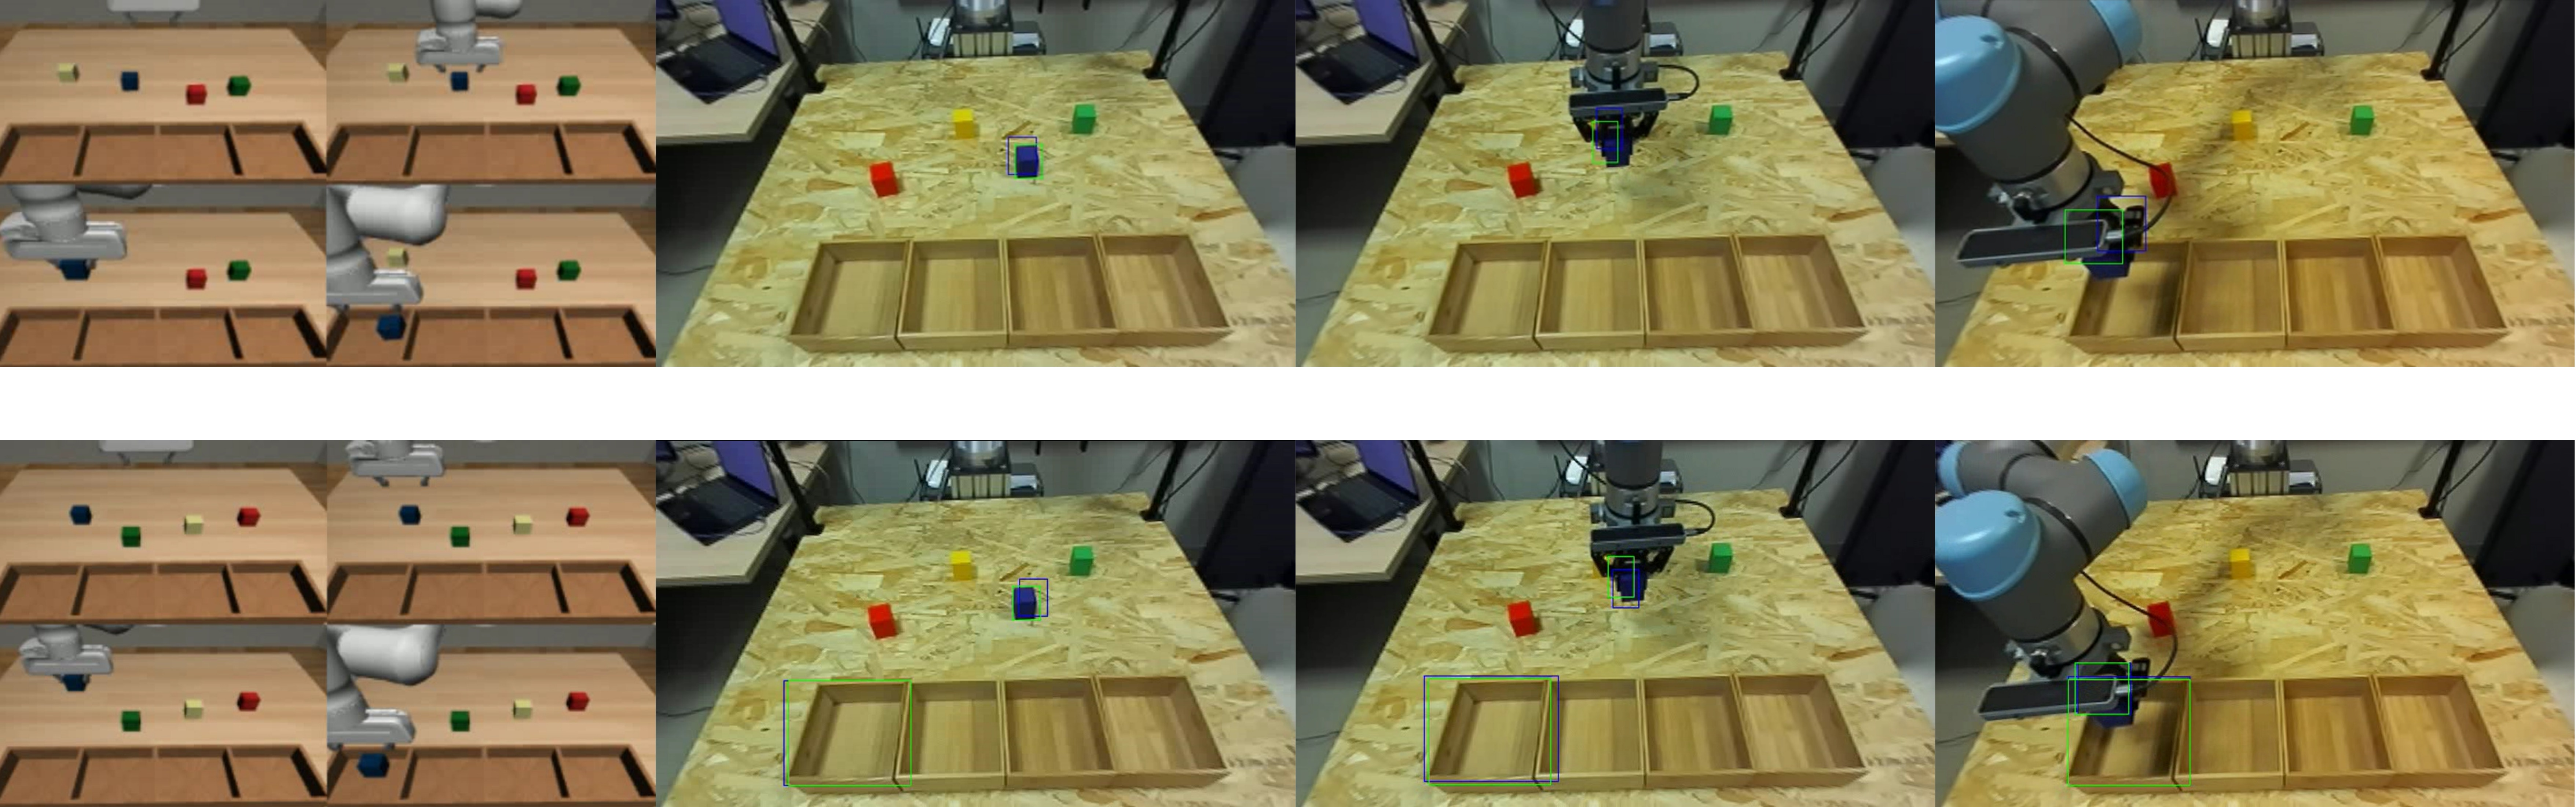
\includegraphics[width=1.0\textwidth]{figures/images/ch5/ctod_cod_prediction.jpg}
    \caption{(Top Row) Example of CTOD prediction. The image shows one of the system the least accurate predictions. While it successfully identifies the target object (blue bounding box), the prediction lacks precision compared to the ground truth (green bounding box). As shown, the offset error increases during placement, likely due to the object being occluded by the gripper. Additionally, some inaccuracies in the ground truth result from the automatic generation process. (Bottom Row) }
    \label{fig:ctod_cod_prediction}
\end{figure}


\paragraph*{MOSAIC-C(T)OD(-P) Validation}\mbox{}\\
In this section, the validation of the MOSAIC-C(T)OD(-P) modules is going to be discussed. The systems have been trained in two different settings: first, with the model trained from scratch using only real-world data, and second, with the model fine-tuned starting from a model initially trained in the simulated environment.

Table \ref{table:ocpl_real_word} summarizes the obtained results. Specifically, these results are based on 10 rollouts per variation, each starting from different initial configurations. Throughout the tests, the aim was to maintain consistency in the scenarios presented while also introducing new scenarios not encountered during training. The evaluation metrics remain the same as those used in Section \ref{sec:ocpl_results}, with a focus on the \textit{Reaching}, \textit{Picking}, and \textit{Success} metrics.
% \usepackage{graphicx}
% \usepackage{multirow}
% \usepackage{hhline}


\begin{table}[t]
    \centering
    \caption{Results obtained by the MOSAIC-C(T)OD(-P) models tested in the real-wolrd sceanrio. For each model two variants are proposed, the first one with the model trained from scratch, the second one with the model finetuned from a simulated trained one.}
    \label{table:ocpl_real_word}
    \resizebox{\linewidth}{!}{%
    \begin{tabular}{|c|c|c|c|c|} 
    \hline
    \textbf{Task} & \textbf{Method} & \begin{tabular}[c]{@{}c@{}}\textbf{Reaching}\\{[}\%]\end{tabular} & \begin{tabular}[c]{@{}c@{}}\textbf{Picking}\\{[}\%]\end{tabular} & \begin{tabular}[c]{@{}c@{}}\textbf{Success}\\{[}\%]\end{tabular} \\ 
    \hhline{|=====|}
    \multirow{5}{*}{\begin{tabular}[c]{@{}c@{}}Pick-Place\\(scratch)\end{tabular}} & MOSAIC & 11.29 & 0.00 & 0.00 \\ 
    \cline{2-5}
     & \begin{tabular}[c]{@{}c@{}}\textbf{\textit{MOSAIC-CTOD}}\\\textbf{\textit{(proposal)}}\end{tabular} & 95.00 & 11.66 & 5.00 \\ 
    \cline{2-5}
     & \begin{tabular}[c]{@{}c@{}}\textbf{\textit{MOSAIC-CTOD-P}}\\\textbf{\textit{(proposal)}}\end{tabular} & 100.00 & 30.00 & 30.00 \\ 
    \cline{2-5}
     & \begin{tabular}[c]{@{}c@{}}\textbf{\textit{MOSAIC-COD}}\\\textbf{\textit{(proposal)}}\end{tabular} & 86.66 & 16.66 & 16.66 \\ 
    \cline{2-5}
     & \begin{tabular}[c]{@{}c@{}}\textbf{\textit{MOSAIC-COD-P}}\\\textbf{\textit{(proposal)}}\end{tabular} & 55.36 & 21.43 & 12.50 \\ 
    \hhline{|=====|}
    \multirow{5}{*}{\begin{tabular}[c]{@{}c@{}}Pick-Place\\(finetuned)\end{tabular}} & MOSAIC & 16.95 & 0.00 & 0.00 \\ 
    \cline{2-5}
     & \begin{tabular}[c]{@{}c@{}}\textbf{\textit{MOSAIC-CTOD}}\\\textbf{\textit{(proposal)}}\end{tabular} & 93.22 & 44.07 & 33.90 \\ 
    \cline{2-5}
     & \begin{tabular}[c]{@{}c@{}}\textbf{\textit{MOSAIC-CTOD-P}}\\\textbf{\textit{(proposal)}}\end{tabular} & 81.36 & 47.46 & 44.07 \\ 
    \cline{2-5}
     & \begin{tabular}[c]{@{}c@{}}\textbf{\textit{MOSAIC-COD}}\\\textbf{\textit{(proposal)}}\end{tabular} & 86.67 & 55.00 & \textbf{55.00} \\ 
    \cline{2-5}
     & \begin{tabular}[c]{@{}c@{}}\textbf{\textit{MOSAIC-COD-P}}\\\textbf{\textit{(proposal)}}\end{tabular} & 85.00 & 46.67 & 46.67 \\
    \hline
    \end{tabular}
    }
    \end{table}

Several observations can be drawn from these results. First, for models trained from scratch, the overall system performance is poor, with a maximum success rate of 30\%. However, the robot demonstrates a high \textit{Reaching-Rate}, which is consistently above 80\%. This suggests that the object prior is effective in informing the control policy about the object's position, even when trained with limited and noisy data. 

The most common failure mode is evident in the drop between the \textit{Reaching} and \textit{Picking} rates, which is primarily due to the gripper colliding with the target object during the picking phase (Figure \ref{fig:robot_rollout}). This issue can be attributed to several factors: one major reason is the precision of the predicted bounding box, which may cause slight misalignment (by a few centimeters) of the gripper, resulting in a collision. Furthermore, the limited and noisy trajectories exacerbate the problem. Even with a correct bounding box, the noisy nature of the trajectories, combined with the probabilistic nature of the policy, can lead to high-variance actions, increasing the likelihood of collisions.
\begin{figure}[t]
    \centering
    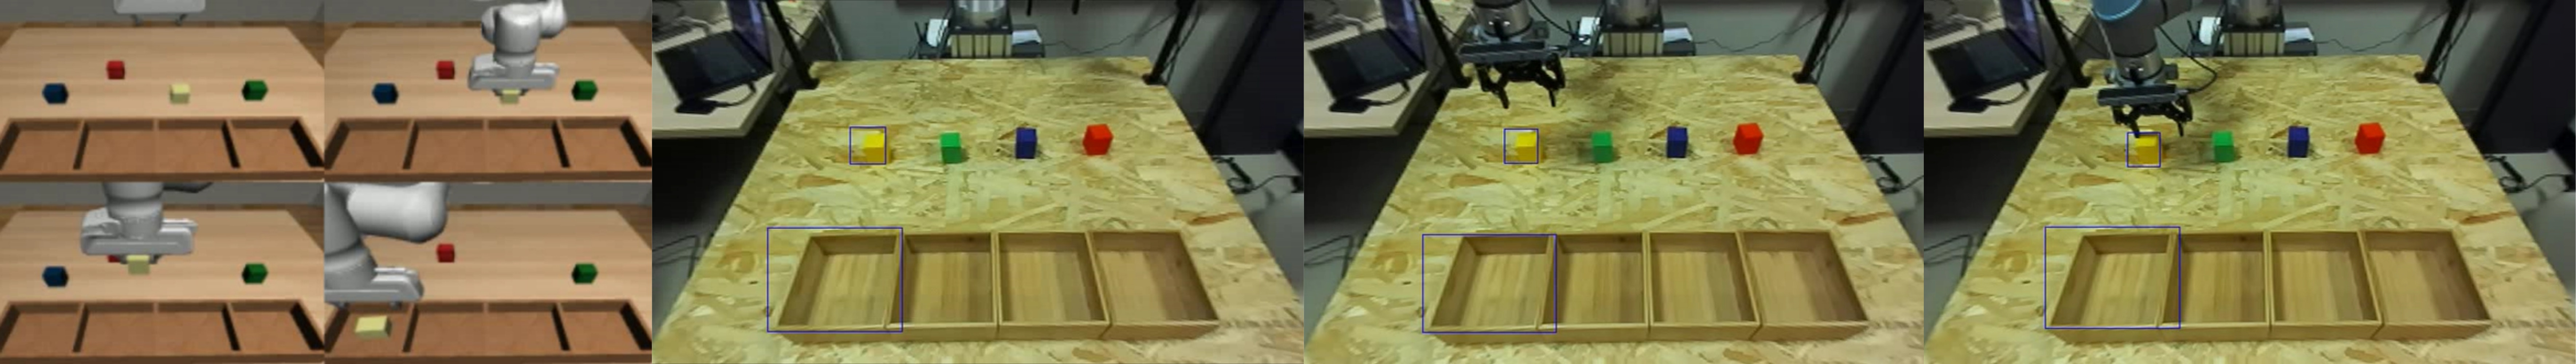
\includegraphics[width=1.0\textwidth]{figures/images/ch5/robot_rollout.jpg}
    \caption{An example of a collision with the target object. This represents the most significant and relevant error mode in the proposed real-world system. As observed, the COD module successfully identifies both the target object and its intended placement location. However, the control module fails to complete the pick operation due to a collision.}
    \label{fig:robot_rollout}
\end{figure}


To address these limitations, a fine-tuned model was introduced. This model leverages the initialization from a simulation-trained model, where the workspace coverage includes less noisy trajectories. As shown in Table \ref{table:ocpl_real_word}, the fine-tuned model significantly improves performance, with the highest success rate (\textbf{55.00\%}) achieved by the MOSAIC-COD module. All fine-tuned models outperform their scratch-trained counterparts. This supports the earlier observation regarding the control module's importance. With proper initialization, the fine-tuned model is better equipped to handle variations in object placement during testing, owing to the improved trajectories from the simulated environment.

% \smalltodo{add figure}